\section{Análisis de Gradientes}

El monitoreo del flujo de gradientes durante el entrenamiento es fundamental para
diagnosticar problemas de estabilidad numérica en redes recurrentes profundas. En
esta sección se analizan las normas L2 de los gradientes registradas durante los
primeros 100 pasos de entrenamiento para ambos modelos, cuya visualización se
presenta en la Figura~\ref{fig:gradient_norms}.

\subsection{Normas Promedio de Gradientes}

Las normas promedio de gradientes calculadas durante los primeros 100 pasos de
entrenamiento son:

\begin{itemize}
    \item \textbf{LSTM:} $\bar{g}_{\text{LSTM}} = 0.018461$
    \item \textbf{GRU:} $\bar{g}_{\text{GRU}} = 0.061758$
\end{itemize}

Ambas normas se mantienen significativamente por debajo del umbral de gradient
clipping configurado ($\text{max\_norm} = 5.0$), lo que indica que el mecanismo
de recorte no necesitó activarse durante esta fase inicial del entrenamiento.

\subsection{Ausencia de Vanishing y Exploding Gradients}

Para verificar la estabilidad del flujo de gradientes, se evalúan dos condiciones
cuantitativas:

\begin{enumerate}
    \item \textbf{Ausencia de vanishing gradients:} Las normas promedio de ambos
    modelos ($0.018461$ para LSTM y $0.061758$ para GRU) son superiores al umbral
    de $1 \times 10^{-7}$, lo que confirma que los gradientes no se desvanecen
    durante la retropropagación a través del tiempo.
    \item \textbf{Ausencia de exploding gradients:} Las normas promedio son
    inferiores al umbral de clipping de $5.0$, y los valores máximos observados
    por capa (ver Tabla~\ref{tab:grad_norms}) no superan $0.54$ en ningún caso,
    confirmando la ausencia de explosión de gradientes.
\end{enumerate}

Esta estabilidad se logra mediante la combinación de dos mecanismos: las compuertas
internas de las arquitecturas recurrentes y el gradient clipping con norma L2
máxima de $5.0$ aplicado como medida preventiva adicional.

\subsection{Rol de las Compuertas en la Estabilidad de Gradientes}

Las arquitecturas LSTM y GRU incorporan mecanismos de compuertas que regulan el
flujo de información y, consecuentemente, el flujo de gradientes durante la
retropropagación.

\paragraph{LSTM — 3 compuertas:}
\begin{itemize}
    \item \textbf{Compuerta de olvido} ($f_t$): Controla qué información del estado
    de celda anterior se descarta. Al inicializarse con bias $= 1.0$, favorece la
    retención de información y permite un flujo de gradientes directo a través del
    estado de celda $c_t$.
    \item \textbf{Compuerta de entrada} ($i_t$): Regula qué nueva información se
    incorpora al estado de celda. Permite que los gradientes fluyan selectivamente
    hacia las representaciones más relevantes.
    \item \textbf{Compuerta de salida} ($o_t$): Determina qué parte del estado de
    celda se expone como estado oculto. Protege el estado interno de perturbaciones
    externas, manteniendo la estabilidad del gradiente almacenado en la celda.
\end{itemize}

La celda de memoria del LSTM actúa como una ``autopista de gradientes'': el estado
$c_t = f_t \odot c_{t-1} + i_t \odot \tilde{c}_t$ permite que los gradientes
fluyan sin transformaciones multiplicativas excesivas cuando $f_t \approx 1$.

\paragraph{GRU — 2 compuertas:}
\begin{itemize}
    \item \textbf{Compuerta de reset} ($r_t$): Controla cuánta información del
    estado oculto anterior se utiliza para calcular el candidato. Permite al modelo
    ``olvidar'' selectivamente, facilitando la captura de dependencias a corto plazo.
    \item \textbf{Compuerta de actualización} ($z_t$): Balancea entre retener el
    estado anterior y adoptar el nuevo candidato mediante la interpolación
    $h_t = (1 - z_t) \odot h_{t-1} + z_t \odot \tilde{h}_t$. Cuando $z_t \approx 0$,
    el gradiente fluye directamente a través de $h_{t-1}$, previniendo el
    desvanecimiento.
\end{itemize}

El GRU logra una estabilidad comparable al LSTM con una arquitectura más simple
(2 compuertas en lugar de 3), al combinar las funciones de la compuerta de olvido
y entrada del LSTM en una sola compuerta de actualización.

\subsection{Normas de Gradiente por Capa}

La Tabla~\ref{tab:grad_norms} presenta el desglose de las normas de gradiente por
tipo de parámetro y capa para ambos modelos, reportando la media y el valor máximo
observados durante los primeros 100 pasos de entrenamiento.

\begin{table}[H]
\centering
\caption{Normas L2 de gradientes por capa durante los primeros 100 pasos de
entrenamiento. Se reportan la media y el máximo para cada tipo de parámetro en
ambos modelos.}
\label{tab:grad_norms}
\begin{tabular}{llrr}
\toprule
\textbf{Parámetro} & \textbf{Modelo} & \textbf{Media} & \textbf{Máximo} \\
\midrule
\texttt{weight\_ih\_l0} & LSTM & 0.065699 & 0.536250 \\
\texttt{weight\_ih\_l0} & GRU  & 0.136939 & 0.443618 \\
\midrule
\texttt{weight\_ih\_l1} & LSTM & 0.075715 & 0.490322 \\
\texttt{weight\_ih\_l1} & GRU  & 0.105860 & 0.374038 \\
\midrule
\texttt{weight\_hh\_l0} & LSTM & 0.059716 & 0.285495 \\
\texttt{weight\_hh\_l0} & GRU  & 0.024349 & 0.095191 \\
\midrule
\texttt{weight\_hh\_l1} & LSTM & 0.103979 & 0.508858 \\
\texttt{weight\_hh\_l1} & GRU  & 0.026597 & 0.114147 \\
\midrule
\texttt{bias\_ih\_l0}   & LSTM & 0.017125 & 0.061730 \\
\texttt{bias\_ih\_l0}   & GRU  & 0.010952 & 0.037317 \\
\midrule
\texttt{bias\_ih\_l1}   & LSTM & 0.017058 & 0.078603 \\
\texttt{bias\_ih\_l1}   & GRU  & 0.017412 & 0.072023 \\
\midrule
\texttt{bias\_hh\_l0}   & LSTM & 0.017125 & 0.061730 \\
\texttt{bias\_hh\_l0}   & GRU  & 0.005384 & 0.018318 \\
\midrule
\texttt{bias\_hh\_l1}   & LSTM & 0.017058 & 0.078603 \\
\texttt{bias\_hh\_l1}   & GRU  & 0.008961 & 0.036128 \\
\bottomrule
\end{tabular}
\end{table}

Se observan las siguientes tendencias en los datos de la Tabla~\ref{tab:grad_norms}:

\begin{itemize}
    \item Los pesos de entrada (\texttt{weight\_ih}) presentan las normas más altas
    en ambos modelos, ya que conectan directamente con la señal de entrada y
    propagan gradientes desde la función de pérdida.
    \item Los pesos recurrentes (\texttt{weight\_hh}) del LSTM muestran normas
    mayores que los del GRU, reflejando la mayor complejidad del flujo de gradientes
    a través de las 3 compuertas del LSTM.
    \item Los bias presentan las normas más bajas, lo cual es esperado dado que
    son vectores de menor dimensionalidad que las matrices de pesos.
    \item Ningún valor máximo supera $0.54$, confirmando que ambos modelos operan
    en un régimen estable muy por debajo del umbral de clipping ($5.0$).
\end{itemize}

\subsection{Visualización del Flujo de Gradientes}

\begin{figure}[H]
    \centering
    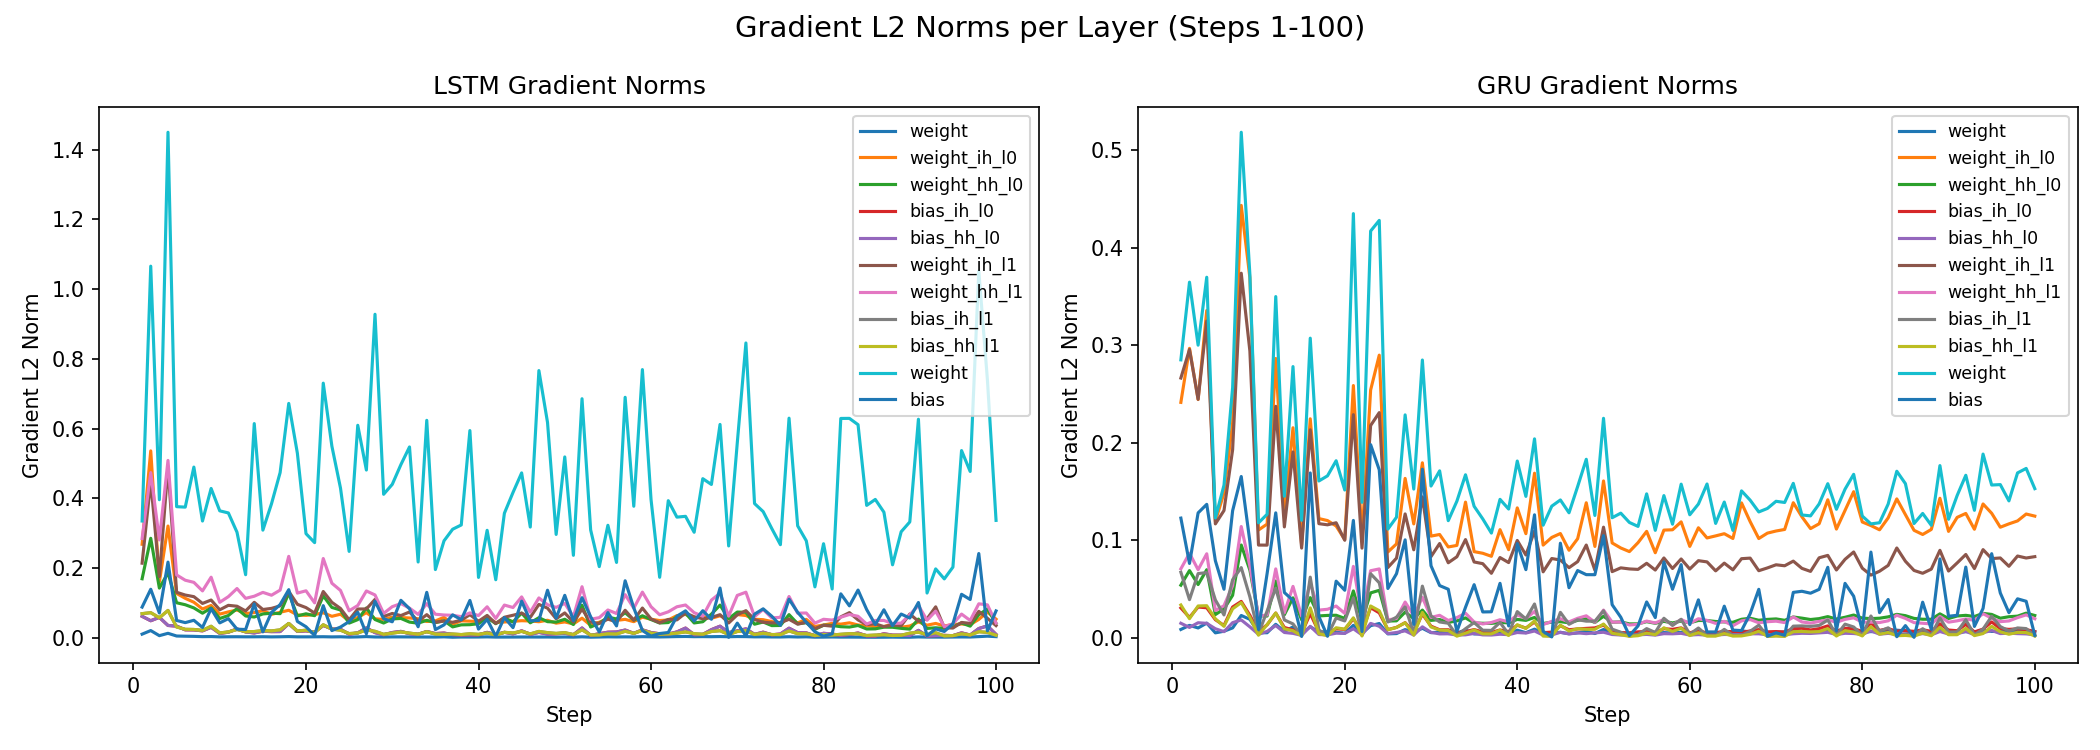
\includegraphics[width=0.9\textwidth]{img/gradient_norms}
    \caption{Normas L2 de gradientes por capa durante los primeros 100 pasos de
    entrenamiento para los modelos LSTM y GRU. Se observa la estabilidad de las
    normas en ambas arquitecturas, sin evidencia de vanishing ni exploding gradients.}
    \label{fig:gradient_norms}
\end{figure}

La Figura~\ref{fig:gradient_norms} confirma visualmente que las normas de gradiente
se mantienen estables a lo largo de los 100 pasos monitoreados, sin tendencias
crecientes (que indicarían explosión) ni decrecientes (que indicarían desvanecimiento).
Ambos modelos exhiben un comportamiento saludable del flujo de gradientes, validando
la efectividad combinada de las compuertas internas y el gradient clipping como
mecanismos de estabilización.
